\chapter{Design}

\section{Overall System Design}

\subsection{Short description of the main parts of the system}

\begin{flushleft}
\textbf{Main Parts of the System}
 \\ \par These are the main parts of the proposed system.
	\begin{itemize}
			\item Proposed System User Interface
			\item Adding a New Job
			\item Adding a New Client
			\item Adding a New Material
			\item Sorting and Searching Clients
			\item Removing Clients or Jobs
			\item Calculating Costs For Each Job
			\item Generate Reports
			\item Invoice Output for Client
			\item Appointment Output for Client
	\end{itemize}

\end{flushleft}


\textbf{Proposed System User Interface}
	\begin{itemize}
		\item Once onto the proposed system, the plasterer will be able to see various buttons in the action bar at the top of the program; these include Add
Jobs, Clients, Materials.
		\item Pressing the Jobs Button will then take them to a different user interface which will then display a series of other options that are applicable under the Jobs section. These include Add Job, Delete Job, Search Jobs, Edit Job. 
		\item 
	\end{itemize}
\textbf{Adding a New Job}

\textbf{Adding a New Client}

\textbf{Adding a New Material}

\textbf{Sorting and Searching Clients}

\textbf{Removing Clients and Jobs}

\textbf{Calculating Costs for each Job}

\textbf{Generate Reports}

\textbf{Invoice Output for Client}

\textbf{Appointment Output for Client}

\subsection{System flowcharts showing an overview of the complete system}

\section{User Interface Designs}

\section{Hardware Specification}

\section{Program Structure}

\subsection{Top-down design structure charts}

\subsection{Algorithms in pseudo-code for each data transformation process}

\subsection{Object Diagrams}

\subsection{Class Definitions}

\section{Prototyping}

\section{Definition of Data Requirements}

\subsection{Identification of all data input items}

\subsection{Identification of all data output items}

\subsection{Explanation of how data output items are generated}

\subsection{Data Dictionary}

\subsection{Identification of appropriate storage media}

\section{Database Design}

\subsection{Normalisation}

\pagebreak
\subsubsection{ER Diagrams}

\begin{figure}[H]
    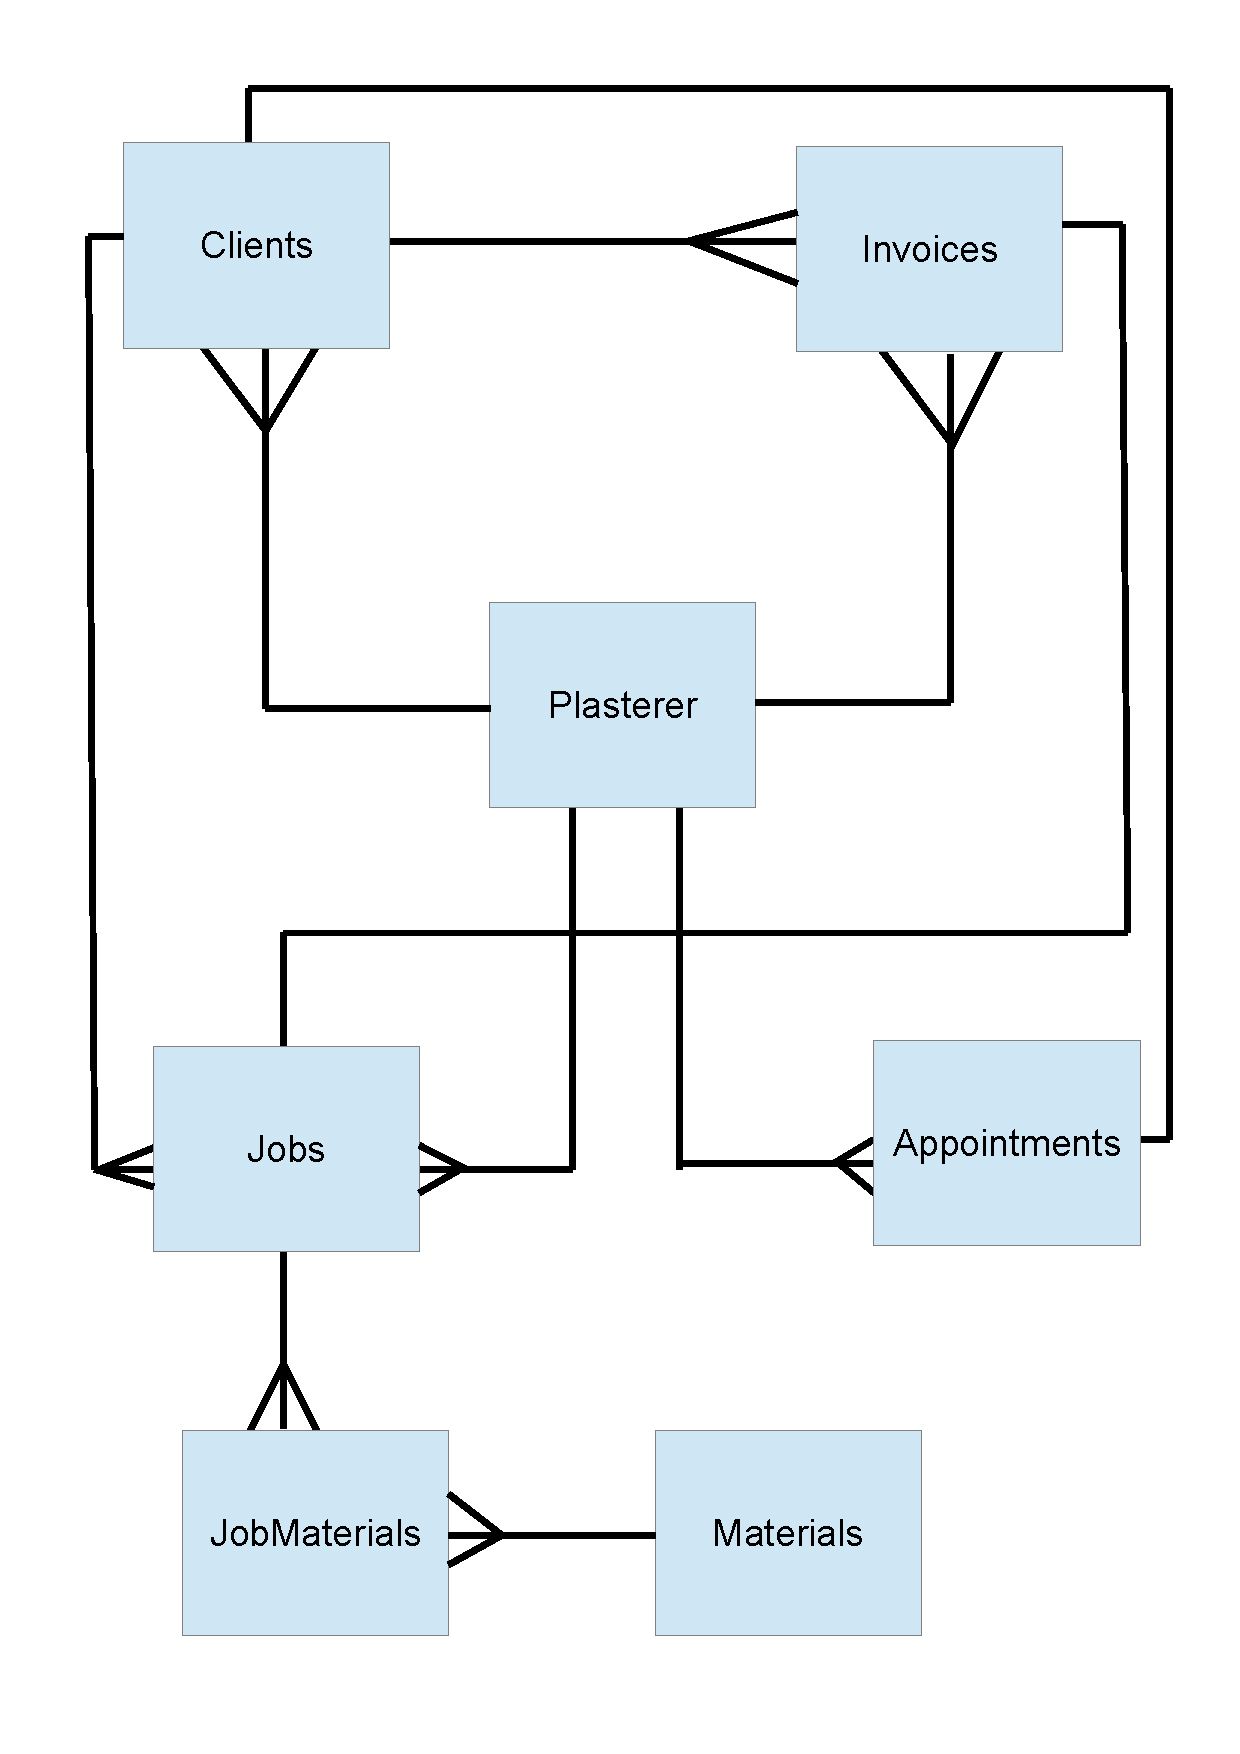
\includegraphics[width=\textwidth]{./Analysis/images/ERDiagram.pdf}
    \caption{This is the entity relationship diagram for the sqlite3 database.} \label{fig:Entity_Relationship_Diagram}
\end{figure}

\subsubsection{Entity Descriptions}

\begin{flushleft}

Below are the entity descriptions for the various entites in the proposed system. An \underline{underlined} attribute denotes a primary key and a \emph{emphasised}	attribute signifies a foreign key in the entity.

\end{flushleft}




\begin{flushleft}
	\textbf{Client}(\underline{ClientID}, ClientTitle, ClientFirstName, ClientSurname, ClientAddrLine1, ClientAddrLine2, ClientAddrLine3, ClientAddrLine4, ClientEmail, ClientPhoneNumber, \emph{PlastererID})
\end{flushleft}



\begin{flushleft}
	\textbf{Plasterer}(\underline{PlastererID}, PlastererFirstName, PlastererSurname, PlastererAddrLine1, PlastererAddrLine2, PlastererAddrLine3, PlastererAddrLine4, PlastererEmail,PlastererPhoneNumber, PlastererDailyRate)
\end{flushleft}



\begin{flushleft}
\textbf{Job}(\underline{JobID}, \emph{ClientID}, \emph{PlastererID}, JobDescription, JobAddrLine1, JobAddrLine2, JobAddrLine3, JobAddrLine4, JobDaysWorked,  JobComplete, JobPaid, \emph{InvoiceID})
\end{flushleft}


\begin{flushleft}
\textbf{Material}(\underline{MaterialID},MaterialName,MaterialPrice)
\end{flushleft}


\begin{flushleft}
\textbf{JobMaterials}(\underline{JobMaterialsID}, \emph{JobID}, \emph{MaterialsID}, JobMaterialsQuantity)
\end{flushleft}


\begin{flushleft}
\textbf{Invoice}(\underline{InvoiceID}, \emph{ClientID}, \emph{JobID}, \emph{PlastererID} InvoiceAmountPreTax, InvoiceAmountAfterTax, InvoiceReceived, InvoiceDate, InvoiceText)
\end{flushleft}



\begin{flushleft}
\textbf{Appointment}(\underline{AppointmentID}, \emph{ClientID}, \emph{PlastererID}, AppointmentDate, AppointmentTime, AppointmentAddrLine1, AppointmentAddrLine2, AppointmentAddrLine3, AppointmentAddrLine4)
\end{flushleft}

\subsubsection{1NF to 3NF}
\begin{flushleft}
    \begin{longtable}{|p{12cm}|}
        \hline
			 \textbf{1NF} \\ \hline
         \textbf{Non-Repeating Attributes} \\ \hline
			PersonID (Primary Key) \\ 
         ClientTitle \\
			ClientFirstName \\
			ClientSurname \\
			ClientAddrLine1 \\
			ClientAddrLine2 \\
			ClientAddrLine3 \\
			ClientAddrLine4 \\
			ClientEmail \\
			ClientPhoneNumber \\
			PlastererTitle \\
			PlastererFirstName \\
			PlastererSurname \\
			PlastererAddrLine1 \\
			PlastererAddrLine2 \\
			PlastererAddrLine3 \\
			PlastererAddrLine4 \\
			PlastererEmail \\
			PlastererPhoneNumber \\
			PlastererDailyRate \\ \hline

			\textbf{Repeating Attributes} \\ \hline
			JobID (Primary Key) \\
			PersonID (Composite Key) \\
          JobDescription \\
			JobAddrLine1 \\
			JobAddrLine2 \\
			JobAddrLine3 \\
			JobAddrLine4 \\
			JobDaysWorked \\
			JobComplete \\
			JobPaid \\
			MaterialName \\
			MaterialPrice \\
			JobMaterialsQuantity \\
			InvoiceAmountAfterTax \\
			InvoiceAmountPreTax \\
			InvoiceReceived \\
			InvoiceDate \\
			InvoiceText \\
			AppointmentDate \\
			AppointmentTime \\
			AppointmentAddrLine1 \\
			AppointmentAddrLine2 \\
			AppointmentAddrLine3	\\
			AppointmentAddrLine4 \\ \hline
			
    \end{longtable}
\end{flushleft}

\begin{flushleft}
    \begin{longtable}{|p{12cm}|}
        \hline
			 \textbf{2NF} \\ \hline
         \textbf{Group} \\ \hline
			PersonID (Primary Key) \\ 
          ClientTitle \\
			ClientFirstName \\
			ClientSurname \\
			ClientAddrLine1 \\
			ClientAddrLine2 \\
			ClientAddrLine3 \\
			ClientAddrLine4 \\
			ClientEmail \\
			ClientPhoneNumber \\
			PlastererTitle \\
			PlastererFirstName \\
			PlastererSurname \\
			PlastererAddrLine1 \\
			PlastererAddrLine2 \\
			PlastererAddrLine3 \\
			PlastererAddrLine4 \\
			PlastererEmail \\
			PlastererPhoneNumber \\
			PlastererDailyRate \\ \hline

			\textbf{Group} \\ \hline
			JobID (Primary Key) \\
			PersonID (Composite Key) \\
         JobDescription \\
			JobAddrLine1 \\
			JobAddrLine2 \\
			JobAddrLine3 \\
			JobAddrLine4 \\
			JobDaysWorked \\
			JobComplete \\
			JobPaid \\ \hline
		
			\textbf{Group} \\ \hline
			JobID (Primary Key) \\ 
			MaterialName \\
			MaterialPrice \\
			JobMaterialsQuantity \\

			\textbf{Group} \\ \hline
			PersonID (Primary Key) \\
			InvoiceAmountAfterTax \\
			InvoiceAmountPreTax \\
			InvoiceReceived \\
			InvoiceDate \\
			InvoiceText \\
			AppointmentDate \\
			AppointmentTime \\
			AppointmentAddrLine1 \\
			AppointmentAddrLine2 \\
			AppointmentAddrLine3	\\
			AppointmentAddrLine4 \\ \hline


    \end{longtable}
\end{flushleft}
\begin{flushleft}
    \begin{longtable}{|p{12cm}|}
                \hline
 			\textbf{3NF} \\ \hline
         \textbf{Group} \\ \hline
			PersonID (Primary Key) \\ 
         ClientTitle \\
			ClientFirstName \\
			ClientSurname \\
			ClientAddrLine1 \\
			ClientAddrLine2 \\
			ClientAddrLine3 \\
			ClientAddrLine4 \\
			ClientEmail \\
			ClientPhoneNumber \\
			PlastererTitle \\
			PlastererFirstName \\
			PlastererSurname \\
			PlastererAddrLine1 \\
			PlastererAddrLine2 \\
			PlastererAddrLine3 \\
			PlastererAddrLine4 \\
			PlastererEmail \\
			PlastererPhoneNumber \\
			PlastererDailyRate \\ \hline

			\textbf{Group} \\ \hline
			JobID (Primary Key) \\
			PersonID (Composite Key) \\
         JobDescription \\
			JobAddrLine1 \\
			JobAddrLine2 \\
			JobAddrLine3 \\
			JobAddrLine4 \\
			JobDaysWorked \\
			JobComplete \\
			JobPaid \\ \hline
		
			\textbf{Group} \\ \hline
			JobID (Primary Key) \\ 
			MaterialID (Foreign Key) \\
			JobMaterialsQuantity \\ \hline


			\textbf{Group} \\ \hline
			MaterialID (Primary Key) \\
			MaterialName \\
			MaterialPrice \\ \hline


			\textbf{Group} \\ \hline
			InvoiceID (Primary Key) \\
			InvoiceAmountAfterTax \\
			InvoiceAmountPreTax \\
			InvoiceReceived \\
			InvoiceDate \\ 
			InvoiceText \\	\hline

		\textbf{Group} \\ \hline 
			AppointmentID (Primary Key) \\
			AppointmentDate \\
			AppointmentTime \\
			AppointmentAddrLine1 \\
			AppointmentAddrLine2 \\
			AppointmentAddrLine3	\\
			AppointmentAddrLine4 \\ \hline


			\textbf{Group} \\ \hline
			PersonID (Primary Key) \\
			AppointmentID (Foreign Key) \\
			InvoiceID (Foreign Key) \\ \hline

			
    \end{longtable}
\end{flushleft}




\section{Security and Integrity of the System and Data}

\subsection{Security and Integrity of Data}

\subsection{System Security}

\section{Validation}

\section{Testing}

\begin{landscape}
\subsection{Outline Plan}

\begin{center}
    \begin{tabular}{|p{2cm}|p{5cm}|p{5cm}|p{4cm}|}
        \hline
        \textbf{Test Series} & \textbf{Purpose of Test Series} & \textbf{Testing Strategy} & \textbf{Strategy Rationale}\\ \hline
        Example & Example & Example & Example \\ \hline
    \end{tabular}
\end{center}

\subsection{Detailed Plan}

\begin{center}
    \begin{longtable}{|p{1.5cm}|p{2.5cm}|p{2.5cm}|p{2cm}|p{2cm}|p{2cm}|p{2cm}|p{2cm}|}
        \hline
        \textbf{Test Series} & \textbf{Purpose of Test} & \textbf{Test Description} & \textbf{Test Data} & \textbf{Test Data Type (Normal/ Erroneous/ Boundary)} & \textbf{Expected Result} & \textbf{Actual Result} & \textbf{Evidence}\\ \hline
        Example & Example & Example & Example & Example & Example & Example & Example \\ \hline
    \end{longtable}
\end{center}
\end{landscape}
